\chapter{Geometry Proposals}

\section{Introduction to dimension matching}

Although Reversible Jump MCMC~\cite{GREEN1995} provides a very general and convenient framework for sampling spaces with varying dimensionality, there are still many practical and problem-specific considerations.
%
Neglecting other components of the acceptance probability, the contribution to the acceptance probability involving dimension matching in the proposal from $(x_{old}, k) \rightarrow (x_{new}, k')$ is given by

\begin{equation} \label{eq:geometry}
    \ln P_\mathrm{geometry} = \left[-u_{k'}(x_{new}) + u_{k}(x_{old})\right] + ln\frac{\phi (x_{old}~|~x_{new})}{\phi (x_{new}~|~x_{old})}
\end{equation}
%
where $u_{k'}$ is the reduced potential for chemical state $k'$, $u_k$ is the reduced potential for chemical state $k$, $x_{new}$ is the new proposed configuration, $x_{old}$ is the old configuration, and $\phi(x,y)$ is the dimension matching distribution.
%
Notably, $x_{new}$ and $x_{old}$ can have different dimensionalities.
%
Intuitively, this involves ensuring that the spaces on which the proposal and the current distribution lie are the same.
%
In other words, we must augment each probability distribution with another distribution that contributes the missing degrees of freedom for each.
%
However, although the recipe is in principle straightforward, it is difficult to construct an efficient dimension matching distribution for the case of chemical space sampling.
%
Among the challenges for constructing an efficient distribution are the multimodality of the target distribution, the need to draw an exact sample, and the need to be able to calculate a normalized probability for the proposal.
%
\section{Problems faced by dimension matching in chemical space}
%
\subsection{The target is highly multimodal}
%
Consider a flexible alkane: a terminal methyl group could be rotated to produce configurations of roughly even probability.
%
Although one might not consider this to be a significant problem, consider the terms in Eq.~\ref{eq:geometry}.
%
The positive contribution of the reverse proposal probability (that is, the probability of placing the atoms being deleted where they were found) means that the proposal distribution must not simply place atoms in a favorable position; it must also recognize favorable positions as such.
%
To use a more concrete example, consider the pair of distributions in Figure~\ref{fig:1D-geometry}. 
%
Although the proposal distribution would clearly place a sample in a favorable location, a sample drawn from the target (such as from a Langevin dynamics simulation) would likely have low probability under the proposal.
%
\begin{figure}[h]
    \centering
    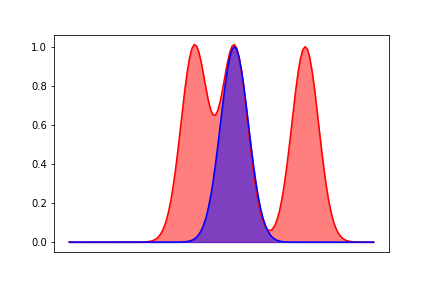
\includegraphics[width=1.0\textwidth]{unimodal.png}
    \caption{An example of a unimodal proposal (blue) with a multimodal target(red). Note that there are many regions of the target that are poorly covered by the proposal.}
    \label{fig:1D-geometry}
\end{figure}
%
This prevents algorithms that, for instance, use a single reference torsion for proposals.
%
As a result of these complex interactions and multimodal distributions, many simple sampling schemes are ruled out.
%
\subsection{The proposal must be drawn exactly}
%
Another choice that may seem attractive is to simply run an MCMC chain for the missing degrees of freedom and use that sample for the new coordinates.
%
However, in order for this to be drawn \emph{exactly} from the target distribution, the Markov chain would have to be run infinitely long (except in the case of perfect MCMC \cite{brooks2011handbook}, which is not applicable here).
%
This is clearly infeasible, and leaves us without familiar tools that we use to sample high-dimensional multimodal probability distributions.
%
\subsection{The proposal must be associated with a normalized probability}
%
Yet another temptation at this point may be to simply draw from a tractable distribution as in the Hastings algorithm~\cite{Hastings1970} (for example, a Gaussian), and then minimize the configuration's energy.
%
However, performing such a nonlinear transformation on the proposed configuration would require that we be able to invert and differentiate the transformation--the determininant of the Jacobian matrix of the transformation is required to calculate the probability.
%
Since we cannot straightforwardly compute such a Jacobian, techniques involving complex nonlinear transformations are largely impractical in this case.
%
\subsection{Atomic positions are correlated}
Further complicating the matter is the fact that various degrees of freedom in a molecule are correlated.
%
For instance, steric hindrance prevents atoms from being placed close to one another.
%
This means that although \emph{a priori} an atom might have a multimodal probability distribution, conditioned on a previous atom, some modes are now precluded.
%
\subsection{Propose one atom at a time}
%
Since proposing a set of atoms at once is fraught with difficulty as described above, one alternative is to propose one atom at a time, significantly reducing the dimensionality of the proposal distribution.
%
However, the challenges described above (especially multimodality and correlated atomic positions) still remain.
%
Following other literature in Grand Canonical Monte Carlo (GCMC) \cite{Siepmann1992} as well as in other molecular simulation literature and statistical literature~\cite{COMBE2003}, we propose positions in so-called internal coordinates.
%
In this coordinate system, atomic positions are defined by a bond length $r$, a bond angle $\theta$, and a dihedral angle $\phi$ as described in Figure~\ref{fig:internal}.
%
\begin{figure}
    \centering
    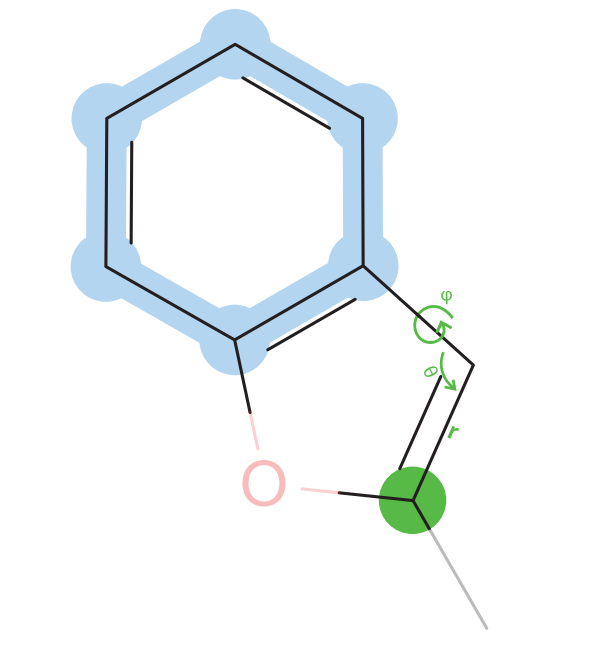
\includegraphics[width=0.4\textwidth]{internalcoords.png}
    \caption{An example of an internal coordinate description of atomic positions. The atom highlighted in green is being proposed, based on the bond (r), angle ($\theta$), and torsion ($\phi$).}
    \label{fig:internal}
\end{figure}
%
\subsection{Naive bond/angle/torsion doesn’t work}
%
Having moved to internal coordinates, the most obvious proposal scheme would be to choose a dihedral angle associated with each atom, and directly propose a bond length, bond angle, and dihedral angle based on the forcefield parameters.
%
However, this has a major pitfall: Although it works with simple geometries and cases where very few atoms need to be added, it fails quickly with complex geometries such as rings, as well as cases where many atoms must be added.
%
In the latter case, one can imagine that neglecting other dihedral and bond angle terms can easily lead to very unfavorable configurations for complex molecules.
%
As a refinement of this algorithm, we include other angle, dihedral, and even nonbonded terms in the proposal scheme.
%
\section{CBMC-like Algorithm}
%
For the common dimension-matching tasks, I implemented and refined a CBMC-like \cite{Siepmann1992, Andrieu2010pmcmc, COMBE2003} algorithm that can take into account forcefield terms besides one bond, angle, and torsion term. 
%
\subsection{Description of algorithm}
The CBMC-like algorithm with guide torsions has several components as follows.
%
At a high level, for a given transformation $k \longrightarrow k'$:
%
\begin{itemize}
    \item Determine which degrees of freedom, based on the atom map, are present in $k'$ not not $k$
    \item Separate atomic degrees of freedom into heavy atoms and hydrogens
    \item Perform a breadth-first search of the molecular graph, identifying the order in which heavy atoms can be proposed
    \item Repeat for hydrogen atoms
    \item For each new atom, propose a bond length, bond angle, and dihedral angle, and convert to cartesian coordinates
    \item Accumulate the log probability of the acceptance probability (described in detail below)
\end{itemize}
%
\subsubsection{Determining the atomic proposal order}
%
After determining which atoms are not mapped, the dimension-matching algorithm must first determine the order in which to propose the new atoms, as well as which internal frame of reference will be used.
%
In greater detail, beginning with a $\ln P_\mathrm{choice} = 0$, a set of atoms with positions and without positions, and until all new atoms are added:
\begin{itemize}
    \item Add atoms which do not have positions, but are connected to a bond, angle, and dihedral partner with positions to atoms\_eligible\_for\_proposal
    \item Uniformly choose without replacement atoms from the atoms\_eligible\_for\_proposal list, and add the probability of choosing each atom to $\ln P_\mathrm{choice}$
    \item For each atom that is chosen, uniformly choose a dihedral angle, and add the probability of this to $\ln P_\mathrm{choice}$
    \item Add each atom that is chosen to atoms\_with\_positions
\end{itemize}
%
The above algorithm is first conducted for the heavy atoms, and then for the hydrogens.
%
When the reverse proposal probability is being evaluated, the same procedure is repeated with stochasticity.
%
It is noteworthy to add here that the use of this algorithm for determining proposal order imposes an extra requirement on the atom map: it must contain at least one atom with a dihedral that can be used for proposal.
%
%
\subsubsection{Coordinate proposal algorithm}
%
Once the proposal order and the reference frame for each atom has been chosen, the algorithm can now stochastically propose coordinates for the new atoms.
%
For each new atom, along with its corresponding dihedral, the proposal algorithm works as follows:
%
\begin{itemize} \label{geometry_algorithm}
    \item If the bond is not constrained, propose bond length $r \sim p(r)=\mathcal{N}(r_0, \sigma^2_r)$, where $\mathcal{N}(\mu, \sigma^2)$ denotes the normal density with mean $\mu$ and variance $\sigma^2$, and $\sigma_r = (\beta K_r)^{-1/2}$ where $K_r$ is the bond force constant; if the bond is constrained, set $r$ to its constraint length $r_0$
    \item Propose bond angle $\theta \sim \mathcal{N}(\theta_0, \sigma^2_\theta)$, where $\sigma_\theta = (\beta K_\theta)^{-1/2}$, where $K_\theta$ is the angle force constant
    \item Propose dihedral angle $\phi \sim p(\phi; r, \theta)$, where $p(\phi ; r, \theta)$ is defined below
    \item Calculate $(x, y, z), \ln \det J(r, \theta, \phi) \longleftarrow$ internal\_to\_cartesian, where $J(r, \theta, \phi)$ is the Jacobian describing the hypervolume $dx \, dy \, dz$ given $dr \, d\theta \, d\phi$, where internal\_to\_cartesian converts from internal coordinates to cartesian coordinates.
    \item Compute the log contribution to the acceptance probability, $\ln P_\mathrm{atom} = \ln \left[ p(r) \, p(\theta) \, p(\phi; r, \theta) \, J(r, \theta, \phi) \right]$

\end{itemize}
%
Note that in Algorithm~\ref{geometry_algorithm}, we are able to use the forcefield's distribution (harmonic) for the bond and angle terms. 
%
However, the dihedral conditional density $p(\phi; r, \theta)$---in the absence of any other nonbonded interactions involving the placed atom---has the form
%
\begin{eqnarray}
p(\phi; r, \theta) &\propto& \exp\left[ -\beta \sum_{l=1}^L \frac{K_{\phi,l}}{2} cos(n_l \phi + \gamma_l) \right]
\end{eqnarray}
%
which does not have a closed-form normalizing constant; here, $K_{\phi,l}$ is a barrier height, $n_l$ is an integral periodicity, and $\gamma_l$ is a phase for the $l$th Fourier term.
%
It is straightforward to numerically normalize this, however, and draw samples using rejection sampling, since the distribution is only one dimensional.
%
Simply drawing from the conditional dihedral term is attractive, but generally affords poor performance, as it neglects most other terms.
%
For linear alkanes and small additions, this approach is feasible.
%
However, for more complex molecules, this approach suffers from several drawbacks. 
%
First, it neglects other valence terms such as the other dihedrals and angles in which the atom in question is involved.
%
Second, it will very often fail to properly create rings, since without the full set of bonds, intermediate dihedral angles would be just as likely to leave the ring open, causing extremely unfavorable valence interactions.
%
Finally, it does not afford the dimension matching scheme an opportunity to incorporate local nonbonded terms.
%
\subsubsection{Improvements to dihedral proposal density}
%
Rather than simply normalizing a single dihedral term and proposing from that, one can instead perform a drive of the angle about its dihedral, and compute the potential energy at each point.
%
This potential may be the full potential, or, for efficiency reasons, a subset of the full potential.
%
Then, having performed the dihedral scan, one can normalize the resulting potential to form a proposal density.
%
An additional hyperparameter of this algorithm is how finely discretized the dihedral angles must be.
%
\subsection{Performance on simple cases}
%
There are a number of different transformations that could be examined.
%
\subsubsection{Substituted Benzenes}
%
Among the simplest are transformations between different substituted benzenes as shown in Figure~\ref{fig:sub_benz}
%
These transformations are straightforward since the molecules are fairly rigid, and there are only several atoms to insert.
%
\begin{figure}
    \centering
    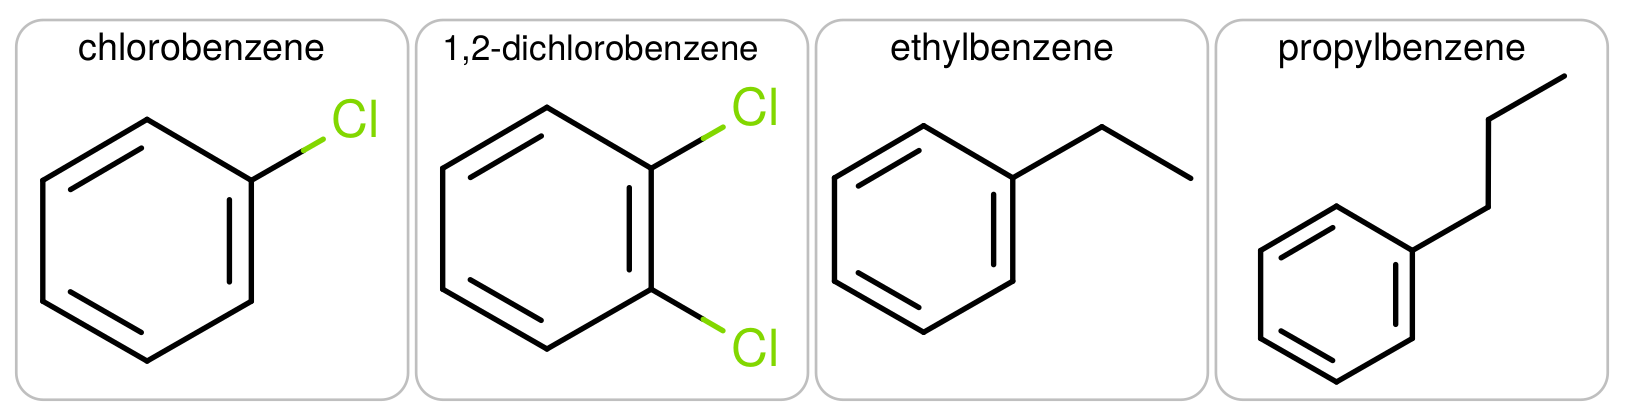
\includegraphics[width=1.0\textwidth]{subs_benz.png}
    \caption{Examples of substituted benzenes}
    \label{fig:sub_benz}
\end{figure}
%
\subsubsection{Alkanes}
%
Another type of transformation that is relatively straightforward is that between alkanes, as shown in Figure~\ref{fig:n-alkanes}.
%
However, these molecules are more flexible, and thus the dimension matching distribution must accurately capture the multimodality of the configurational probability distribution.
%
\begin{figure}
    \centering
    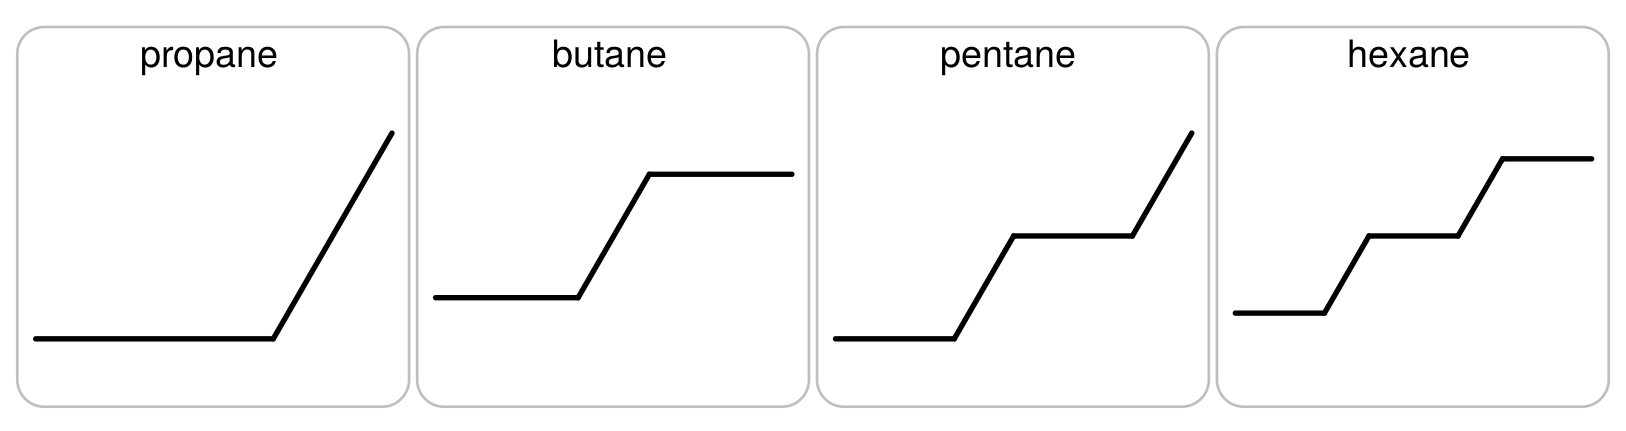
\includegraphics[width=1.0\textwidth]{alkanes.png}
    \caption{Examples of n-alkanes}
    \label{fig:n-alkanes}
\end{figure}
%
\subsubsection{More complex transformations}
%
Of course, while alkanes and substituted benzenes are useful model systems and the building blocks of many interesting compounds, we are far more interested in complex transformations, such as the addition of rings or jump between different drug-like molecules.
%
In order to achieve these, however, we must further improve our strategy.
%
One immediate difficulty, even with the improved dihedral scan, is that building a ring will often result in failure.
%
The failure to close a ring results from the fact that when the intermediate ring atoms are being inserted, there are no terms that cause the ring to close, resulting in a grotesque geometry.
%
To remedy this, we can add "guide torsions" that encourage the ring to close by removing the dihedral modes that correspond to an open ring as in~\cite{Wick2000}.
%
The algorithm for the addition of guide torsions works as follows:
\begin{itemize} \label{ringclosure}
    \item Convert the molecule into the OpenEye OEMol format
    \item Perceive rigid bonds
    \item Generate a reference configuration using OpenEye Omega
    \item Measure the dihedral angles about the rigid bonds
    \item Add a dihedral term with a mode at the angle in the reference conformation
\end{itemize}
%
By applying the steps in Algorithm~\ref{ringclosure}, we can significantly increase the chance of proposing a closed ring, resulting in a more realistic geometry.
%
\subsection{Shortcomings}
%
However, with very large changes (involving the addition of many atoms), this approach is still not terribly performant.
%
As an example of Sequential Importance Sampling (SIS), it suffers from the compounding of poor choices made earlier in the sequence.
%
As the number of degrees of freedom that must be added grows, this problem becomes more serious, demonstrated in Figure~\ref{fig:dof_added_worse}.
%
\begin{figure}
    \centering
    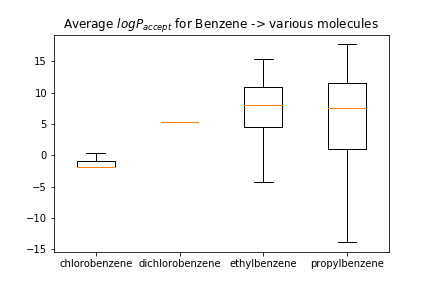
\includegraphics{dof_demo.png}
    \caption{The average $\ln P_\mathrm{accept}$ \emph{vs.} the number of degrees of freedom added. 
    Note that the variance is quite low for small (chlorobenzene and dichlorobenzene) changes, but quickly grows with the addition of flexible chains. Note that anything beyond the 98th percentile was clipped for this figure.}
    \label{fig:dof_added_worse}
\end{figure}
%
When the approach is tried on even more complex transformations, such as between kinase inhibitors, we observe even more severe performance loss, making acceptance a highly unlikely proposition.
%
However, there are yet remedies to these serious problems.
%
\section{Future directions: Particle Filtering}
%
\subsection{Basic Overview}
%
Instead of simply choosing one dihedral angle at each atom in \ref{geometry_algorithm}, we can choose N dihedral angles and calculate an importance weight based on the difference between the probability of that atom's placement under the target distribution.
%
Then, after a specified number of atoms are inserted, the algorithm resamples $N$ of the configurations based on their weights.
%
This technique is called particle filtering \cite{DelMoral1997,Henriksen2012}, and is commonly used in state space models.
%
\subsection{Advantages}
%
Particle filtering can enable the algorithm to eliminate proposals that were reasonable at stage $m$ but become very unfavorable at stage $m+n$.
%
For example, if a “particle” (as the replicates of configurations are known in statistics) does not close a ring, when the ring closure should happen, its weight will be very small and it will be lost in the resampling.
%
On the other hand, naive multinomial resampling carries with it its own risks: since at every resampling step there is a nonzero probability for favorable configurations to be lost, after enough resampling steps, the probability that favorable configurations are lost can grow quite high.
%
Mitigating this are other resampling algorithms, which aim to reduce the deleterious effect of multinomial sampling
%
In addition to these advantages, particle filtering can be parallelized on tightly-coupled parallel hardware such as graphics processors~\cite{lee2010utility}.
%
\subsection{Algorithm Hyperparameters}
%
As briefly mentioned above, the particle filter has a number of hyperparameters that can be tuned and tweaked.
%
Among these are the number of particles or replicates, the method used for resampling, and, as above, the method used for proposing the individual bonds, angles, and dihedrals. 
%
\subsubsection{Number of Particles}
The most obvious algorithm hyperparameter is the number of particles. The larger this number is, the better the performance of the dimension matching algorithm.
%
However, each particle requires the computation of the target density, which can be quite expensive.
%
Because cost scales relatively quickly in this case, it would be ideal to minimize the number of particles needed.
%
Furthermore, a very large number of particles can cause serious numerical instabilities \cite{Murray2016}, primarily from the need to normalize weights before resampling.
%
\subsubsection{Resampling Algorithm}
One can choose various approaches for the resampling step of the particle filter. 
%
The simplest is known as multinomial resampling, and consists of simply drawing $N$ particles with replacement from the previous $N$ according to their weights.
%
This is known to have a relatively high variance \cite{Douc2005}.
%
Another approach is so-called stratified resampling, which 
%
This also requires weight normalization, however.
%
In situations with large numbers of particles, it may be feasible to resort to a scheme that is "almost" exact, such as Metropolis resampling. \cite{Murray2016}
%
In the Metropolis resampling scheme, one proposes to sample a particular ancestor and accepts/rejects.
%
One then repeats this procedure many times until approximate convergence.
%
These steps must be performed at each resampling attempt.
%
This is not technically exact, as Metropolis MCMC only converges in the asymptotic limit, not for finite samples.
%
However, in some studies \cite{Murray2016}, it actually has less bias than the exact methods, because weight normalization is not required and certain numerical issues are resolved
%
Parallelization is also facilitated by Metropolis resampling, since the weights do not need to be normalized (a reduction operation) before resampling.
%
\subsubsection{Overall comparison}
Finally, below is a table which compares the features of various proposal schemes that are in principle correct for the dimension matching algorithm.
%
\begin{table}
\caption{{\bf Comparison of features of various proposal schemes for dimension matching.}
\label{tab:proposal-scheme-comparison}
}
\begin{center}
    \footnotesize
    \begin{tabular}{||c | c | c | c | c | c | c||}
    \hline
         Method & Multimodal & Exact & computable P & Rings & Correlated & Speed \\
         \hline
         Minimization &  Yes & Yes & No & Yes & Yes & Fast \\
         Unimodal & No & Yes & Yes & No & No & Fast \\
         Multi-reference & Yes & Yes & Yes & Yes & No & Fast \\
         CBMC-like & Yes & Yes & Yes & No & Moderate & Moderate \\
         CBMC+guide & Yes & Yes & Yes & Yes & Moderate & Moderate\\
         Particle Filtering & Yes & Yes & Yes & Yes & Yes & Slow \\
         \hline
    \end{tabular}
\end{center}
\end{table}
%
%
\section{Tuning of Dimension Matching Parameters in the context of NCMC}
%
It should be noted that although the parameters for the dimension matching proposal are very important, there are several tradeoffs between tuning the parameters of the dimension matching and those of the NCMC or annealing, described in the next chapter.
%
The implementation details of each are quite different, leading to interesting tradeoffs.
%
For instance, although the energy computations in the dimension matching algorithm are much faster (they exclude the majority of the system's interactions), the annealing runs on the GPU, which often more than compensates for the added terms in the energy computation.
%
An additional point to note is that the dimension matching (especially particle filtering) can be subject to numerical stability issues.
%
Because the annealing protocol is typically very slow, and steps of Langevin Dynamics are taken between changes in the control parameter, the NCMC component of the overall algorithm may be better behaved.
%
For this reason, it is useful to jointly optimize the parameters.
%
\subsection{Tradeoffs}
%
There is to some extent a tradeoff between the hyperparameters of the dimension matching algorithm, and those of the annealing.
%
Intuitively, one might imagine that additional grid points and the use of nonbonded forces in the dimension matching scheme might result in the need for fewer steps of NCMC.
%
However, due to the current setup of the NCMC, this is not terribly helpful.
%
Nonbonded forces are initially disabled for the new atoms (except intramolecular nonbonded forces), and so using the constributions of intermolecular nonbonded forces to proposed new geometries is likely to result in an inferior acceptance probability.
%
As to the number of grid points, this could potentially be reduced with longer NCMC by including valence softening in the NCMC.
%
However, the default configuration of NCMC does not include this, and so the number of grid points is largely decoupled from the NCMC protocol length.
%
However, another potentially fruitful approach is to allow the NCMC code to soften the bonds and angles at the initial value of the control parameter.
%
This allows otherwise unfavorable geometry proposals to be accorded a favorable energy, then slowly anneal back to the forcefield's parameters for those terms.
%
It should be noted that doing this would then introduce a dependency between the geometry proposal's hyperparameters and the NCMC protocol.
%
For example, it may result in the need for longer protocols, or may cause very unfavorable reverse geometry proposal probabilities.
%
To understand the latter point, consider that if the NCMC protocol is symmetric, the atoms to be deleted will conclude the protocol with soft bonds and angles, thus distorting the geometry from what the forcefield would otherwise cause.
%
However, the geometry proposal distribution is simply using the forcefield's parameters, and as such will likely assign low probability to the ending configuration.
%
This can be straightforwardly ameliorated by modifying the geometry engine to also be able to soften its bond and angle proposal distributions, thereby once again matching the distribution seen in the nonequilibrium switching.

